\documentclass{article}

\usepackage{tabulary}
\usepackage{listings}
\usepackage{algorithmicx}
\usepackage{minted}
\usepackage{program}
\usepackage{graphicx}
\usepackage[colorlinks=true,linkcolor=blue]{hyperref}
\usepackage[nochapter]{vhistory}
\usepackage{siunitx}

% If LaTeX just doesn't do what I want, buy http://www.amazon.com/gp/product/0201362996

% Used for tables that can span pages:
\usepackage{xtab}
\tabletail{\hline \multicolumn{4}{|r|}{{Continued on next page}} \\ \hline}

% Keep spacing normal in enumerated instead of adding extra space between
% items.
\usepackage{enumitem}
%\setlist{nolistsep}

\newenvironment{commentary}
{
   \begin{quotation}
   \noindent
   \small \em
   \rule{\linewidth}{1pt}\\
}
{
   \end{quotation}
}

\newenvironment{steps}[1]
{
   \vspace{1ex}
   \noindent
   #1
   \begin{enumerate}[nosep]
}
{
   \end{enumerate}
   \vspace{1ex}
}


% All registers are named here. That way when we rename one we'll get errors if
% there are still references to the old name.
\usepackage{xspace}
\newcommand{\defregname}[2]{\providecommand{#1}{{\tt #2}\xspace}}
\newcommand{\deffieldname}[2]{\providecommand{#1}{{$|#2|$}\xspace}}
\deffieldname{\Fmprv}{mprv}
\defregname{\Rmstatus}{mstatus}

\defregname{\Azero}{a0}
\defregname{\Aone}{a1}

\defregname{\Rzero}{zero}
\defregname{\Szero}{s0}
\defregname{\Sone}{s1}

\defregname{\Tzero}{t0}

\defregname{\Xzero}{x0}
\defregname{\Xone}{x1}
\defregname{\Xeight}{x8}
\defregname{\Xnine}{x9}
\defregname{\Xten}{x10}
\defregname{\Xeleven}{x11}
\defregname{\Xthirtyone}{x31}
\defregname{\Fone}{f1}
\defregname{\Rpc}{pc}
\defregname{\Rmhartid}{mhartid}
\defregname{\Rmepc}{mepc}

\input{hwbp_registers.tex.inc}
\input{core_registers.tex.inc}
\input{jtag_registers.tex.inc}
\input{dm1_registers.tex.inc}
\input{dm2_registers.tex.inc}
\input{trace_registers.tex.inc}
\input{sample_registers.tex.inc}
\input{abstract_commands.tex.inc}

\newcommand{\versionnum}{0.13}
\newcommand{\shortdate}{jan23}
\newcommand{\longdate}{January 23, 2017}

\title{RISC-V External Debug Support\\
Version \versionnum\shortdate}
\author{Tim Newsome \textless tim@sifive.com\textgreater}
\date{\longdate}

\begin{document}
\maketitle

{\bf Warning! This draft specification will change before being accepted as
standard, so implementations made to this draft specification will likely not
conform to the future standard.}

\tableofcontents
\listoffigures
\listoftables

\newpage

\section*{Acknowledgments}

I would like to thank the following people for their time, feedback, and ideas:
Bruce Ableidinger,
Krste Asanovic,
Mark Beal,
Monte Dalrymple,
Peter Egold,
Richard Herveille,
Gajinder Panesar,
Klaus Kruse Pedersen,
Antony Pavlov,
Ken Pettit,
Wesley Terpstra,
Megan Wachs,
Stefan Wallentowitz,
Ray Van De Walker,
Andrew Waterman,
and Andy Wright.

\section{Introduction}

Software contains bugs, and to help find these bugs it is critical to have good
debugging tools. Unless a robust OS is running on a core, with convenient
access to it (eg. over a network interface), hardware support is required to
provide visibility into what is going on in that core.  This document outlines
how that support should be provided on RISC-V platforms.

\section{About This Document}

\subsection{Structure}

This document contains two parts. The main part of the document is the
specification, which is given in the numbered sections. The second part
of the document is a set of  appendices. The information
in the appendix is intended to clarify and provide examples, but is
not part of the actual specification.

\subsection{Terminology}

A \emph{platform} is a single integrated circuit consisting of one or more
\emph{components}.
Some components may be RISC-V cores, while others may have a different
function. Typically they will all be connected to a single system bus.
A single RISC-V core contains one or more hardware threads, called
\emph{harts}.

\subsection{Register Definitions}

All register definitions in this document follow the format shown in Section~\ref{shortname}.
A simple graphic shows which fields are in the register. The
upper and lower bit indices are shown to the top left and top right of each
field. The total number of bits in the field are shown below it.

After the graphic follows a table which for each field lists its name,
description, allowed accesses, and reset value. The allowed accesses are listed
in Table~\ref{tab:access}.

\begin{table}[htp]
    \centering
    \caption{Register Access Abbreviations}
    \label{tab:access}
    \begin{tabulary}{\textwidth}{|l|L|}
        \hline
        R & Read-only. \\
        \hline
        R/W & Read/Write. \\
        \hline
        R/W0 & Read/Write. Only writing 0 has an effect.  \\
        \hline
        R/W1 & Read/Write. Only writing 1 has an effect.  \\
        \hline
        W & Write-only. When read this field returns 0. \\
        \hline
        W1 & Write-only. Only writing 1 has an effect. \\
        \hline
    \end{tabulary}
\end{table}

\input{sample_registers.tex}

\section{Background}

There are two forms of external debugging. The first is \emph{halt mode}
debugging, where an external debugger will halt some or all components of a
platform and inspect them while they are in stasis. Then the debugger can allow
the hardware to either perform a single step or to run freely.

The second is \emph{run mode} debugging.  In this mode there is a software
debug agent running on a component (eg.  triggered by a timer interrupt on a
RISC-V core) which communicates with a debugger without halting the component.
This is essential if the component is controlling some real-time system (like a
hard drive) where halting the component might lead to physical damage. It
requires more software support (both on the chip as well as on the debug
client).  For this use case the debug interface may include simple serial
ports.

A third use for the external debug interface is to use it as a general
transport for a component to communicate with the outside world. For instance,
it could be used to implement a serial interface that firmware could use to
provide a simple CLI. This can use the same serial ports used for run-mode
debugging.

\section{Supported Features}
The debug interface described out here supports the following features:
\begin{enumerate}
   \item RV32, RV64, and future RV128 are all supported.
   \item Any hart in the platform can be independently debugged.
   \item Arbitrary instructions can be executed on a halted hart. That means no
       new debug functionality is needed when a core has custom instructions or
       registers, as long as there exist programs that can store those
       registers to memory.
   \item With optional extensions it becomes possible to halt a core very
       briefly and quickly execute a a few instructions before letting it
       resume.
   \item Memory is accessed through the core, so the debugger will see the same
       thing that the code that is executing sees.
   \item Optionally, a bus master can be implemented to allow memory access
       without involving any hart.
   \item Debugging can be supported over multiple transports.
   \item Code can be downloaded efficiently.
   \item Each hart can be debugged from the very first instruction executed.
   \item A RISC-V core can be halted when a software breakpoint instruction is
       executed.
   \item Hardware can step over any instruction.
   \item A RISC-V core can be halted when a trigger matches the PC, read/write
       address/data, or an instruction opcode.
   \item The debug module may implement serial ports which can be used for
       communication between debugger and monitor, or as a general protocol
       between debugger and application.
   \item The debugger doesn't need to know anything about the microarchitecture
       of the cores it is debugging.
   \item The spec can be implemented without touching a core's data path.
\end{enumerate}

\section{System Overview}

The Debug System is designed to let a debugger feed a halted hart arbitrary
instructions, while keeping gate count to a minimum. This is necessary
functionality, and once it exists it can be used to accomplish all debug tasks.
To speed up certain repetitive operations, an optional Instruction Buffer can
be implemented. This is designed so that debug software can easily take
advantage of it, without needing a separate implementation for when it is and
isn't supported.

Figure~\ref{fig:overview} shows the main components of External Debug Support.
Blocks shown in dotted lines are optional.

\begin{figure}
   \centering
   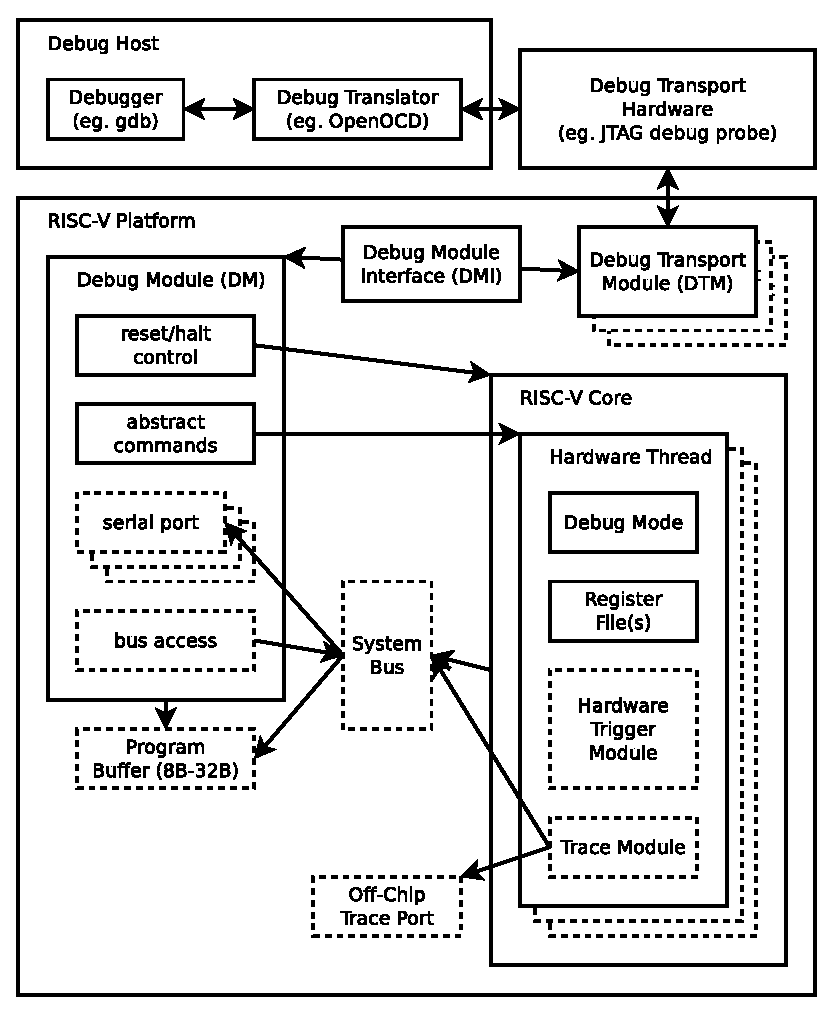
\includegraphics[width=\textwidth]{overview.eps}
   \caption{RISC-V Debug System Overview}
   \label{fig:overview}
\end{figure}

The user interacts with the Debug Host (eg. laptop), which is running a
debugger (eg. gdb).  The debugger communicates with a Debug Translator (eg.
OpenOCD, which may include a hardware driver) to communicate with Debug
Transport Hardware (eg.  Olimex USB-JTAG adapter) that's connected to the host.
The Debug Transport Hardware connects the Debug Host to the Platform's Debug
Transport Module (DTM).  The DTM provides access to the DM using the Debug
Module Interface (DMI).

The DM allows the debugger to halt any hart in the platform.  When a hart is
halted the DM can cause it to execute arbitrary instructions, and the hart can
move data to/from the DM as well.  Optionally the DM can contain an Instruction
Buffer to feed instructions more efficiently. As a further extension a Scratch
RAM may be implemented which can be used to briefly halt a hart and execute a
few instructions without requiring any debugger interaction once the process
has started.

Each RISC-V core may implement a Trigger Module for each hart.  These can
implement breakpoints, which cause a hart to halt spontaneously.  When that
happens the DM notices because the hart will signal the DM that it's ready for
an instruction.

\section{Debug Transport Module (DTM)}

Debug Transport Modules provide access to the DM over one or more transports
(eg. JTAG or USB).

There may be multiple DTMs in a single platform. Ideally every component that
communicates with the outside world includes a DTM, allowing a platform to be
debugged through every transport it supports.  For instance a USB component
could include a DTM. This would trivially allow any platform to be debugged
over USB. All that is required is that the USB module already in use also has
access to the Debug Bus.

Using multiple DTMs at the same time is not supported. It is left to the user
to ensure this does not happen.

\section{Debug Module (DM)} \label{dm}

\begin{steps}{The Debug Module is the interface between specific debug
    operations and their implementation. It must support the following
    operations:}
\item Provide access to a reset signal that resets most of the SoC.
\item Allow any individual hart to be halted.
\item Provide status on which harts are halted.
\item Feed a specific hart one instruction, and have that hart execute the
    instruction.
\item Give the debugger necessary information about the implementation.
\item Provide status on whether a data access is pending.
\item Service a data access (load or store).
\end{steps}

Optionally, an Instruction Buffer can repeatedly feed the same set of
instructions to a hart.

A single DM can debug up to 1024 harts.

\subsection{Debug Module Interface (DMI)}

The Debug Module Interface can be a trivial bus with one master and one slave,
or use a more full-featured bus like TileLink or the AMBA Advanced Peripheral
Bus. The details are left to the system designer.

The DMI uses between 4 and 32 address bits.  It supports read and write
operations, which may return an error. (Errors are only used by the optional
Bus Access and Serial Port blocks.) The bottom of the address space is used for
the DM. Extra space can be used for custom debug devices, other cores,
additional DMs, etc.

The space is laid out so that small systems can get away with just 4 address
bits. Using the Instruction Buffer requires 5 bits, and systems that have many
cores will want to implement 6 bits.

\begin{table}[htp]
    \centering
    \caption{Debug Module Interface Address Space}
    \label{tab:header}
    \begin{tabulary}{\textwidth}{|r|l|}
        \hline
        0x00 -- 0x1f & Registers described in Section~\ref{dmdebbus}. \\
        \hline
        0x20 -- 0x3f & If accessible, there are 1024 bits here, one for each
        hart that may exist in the system. If the hart is ready for the DM to
        feed it an instruction, the bit is 1. Otherwise the bit is 0. The bit
        for hart 0 is the LSB in the 32-bit word at 0x20. The bit for hart 1023
        is the MSB in the 32-bit word at 0x3f. \\
        \hline
    \end{tabulary}
\end{table}


\subsection{Reset Control} \label{reset}

This block is connected to the global reset signal, which resets every
component in the platform except for the Debug Module itself.

\subsection{Halt Control}

This block controls halt signals from the Debug Module to a hart.  It is used
to halt a hart, and let it run again.

For each hart the block contains a single bit that is accessible through to
\Fhalt in \Rdmcontrol. When a debugger wants to halt a hart, it writes 1 to
this bit, and then waits for an instruction fetch to be pending from the hart.
To resume, the debugger clears the bit.

The Debug Module conceptually has a direct connection to the halt signal of
every hart that has one. When set or cleared, a hart must respond in less than
one second.  (How this is implemented is not further specified. A few clock
cycles will be a more typical latency.)

\subsection{Abstract Commands}

A debugger can execute abstract commands by writing the command to \Rcommand.
If a command takes an argument, the debugger must write it to the {\tt data}
registers before writing to \Rcommand. If a command returns a results, it is
placed in the {\tt data} registers when the command is complete.

When debugging a 32-bit core, each argument fits in one {\tt data} register.
When debugging a 64-bit core, each argument uses two {\tt data} registers.
When debugging a 128-bit core, each argument uses four {\tt data} registers.

\begin{table}[htp]
    \centering
    \caption{Abstract Register Numbers}
    \label{tab:regno}
    \begin{tabulary}{\textwidth}{|r|l|}
        \hline
        0x0000 -- 0x0fff & CSRs \\
        \hline
        0x1000 & PC \\
        \hline
        0x1020 -- 0x103f & GPRs \\
        \hline
        0x1040 -- 0x105f & Floating point registers \\
        \hline
    \end{tabulary}
\end{table}

\input{abstract_commands.tex}

\subsection{Data Access / Instruction Fetch}

While most of the language in this spec refers to data accesses and instruction
fetches as if they occur over a bus, this is actually implementation-dependent.
An implementation could feed instructions to a hart some other way, and data
exchange could occur through special CSRs. These details aside, each access
still goes through the same stages as a bus access, so that language is used
here.

When a hart performs an access (data read/write or instruction fetch) to the
DM, this block updates bits in \Raccess. The debugger can then access \Rdaccess
or \Rifetch to complete the access.

\subsection{Instruction Buffer}

This optional block contains between 3 and 7 instructions and a pointer to the
next instruction. If enabled, the DM will automatically complete accesses from
the currently selected hart with the next instruction, and increment the
pointer. When all instructions are executed, the Instruction Buffer may be
disabled, start over at the beginning, or \Fhalt will be cleared.

3 instructions is enough to speed up reading and writing blocks of memory.  5
instructions is enough to read from a given memory address while halting the
processor only briefly.  7 instructions is enough to write to a given memory
address while halting the processor only briefly.

\subsection{Scratch RAM}

This optional block could be used by a debugger to save/restore registers
faster than transmitting them to the debugger.

It could also be used for a quick access, which halts a hart for the minimum
amount of time. The debugger would write a small program to the Instruction
Buffer, and use the Scratch RAM to save/restore registers, pass arguments, and
return a value. See Section~\ref{quickaccess}.

\subsection{Serial Ports}

The Debug Module may implement up to 8 serial ports. They support basic flow
control and full duplex data transfer between a component and the debugger.
They can be used to communicate with a debug monitor running on a hart, for the
equivalent of printf debugging, to provide a simple CLI without requiring any
extra peripherals, or more generally to emulate devices that aren't present.
All these uses require software support, and are not further specified here.

\subsection{Bus Access}

In a minimal configuration a debugger can access the system bus by having a
RISC-V hart perform the accesses it requires. Optionally a Bus Access block may
be implemented. Because the Bus Access block performs accesses directly from
the DM, it only uses physical addresses.

Implementing a Bus Access block has several benefits. First, it is possible to
access memory in a running system with minimal impact.  Second, it may improve
performance when downloading programs. (There is only a benefit if JTAG TCK is a
significant fraction of the RISC-V hart's clock speed.)  Third, it may provide
access to devices that a hart does not have access to. A hart may be unable to
access all devices in a system (eg. for security reasons) and in this case the
debugger needs another path to access them.

To keep implementing, configuring, and using a debugger as simple as possible,
systems should use the same memory map for each hart. That means that a given
address maps to the same device no matter which hart performs the access.
(Different harts may not all have permission to access the same devices.) If
different harts do have unique memory maps then the system should provide
access to all devices using the Bus Access block. This will make implementing,
configuring, and using a debugger more complex so should be avoided if
possible.

\subsection{Security}

To protect intellectual property it may be desirable to lock access to the
Debug Module.  To allow access during a manufacturing process and not
afterwards, a reasonable solution could be to add a fuse bit to the Debug
Module that can be used to be permanently disable it. Since this is technology
specific, it is not further addressed in this spec.

Another option is to allow the DM to be unlocked only by users who  have an
access key. A simple mechanism is documented in Section~\ref{authdata0}. When
\Fauthenticated is clear, the DM must not interact with the rest of the
platform in any way.

\subsection{Debug Module DMI Registers} \label{dmdebbus}

\input{dm1_registers.tex}

\subsection{Debug Module Serial Registers} \label{dmsysbus}

TODO: Figure out where these registers should really live on the system bus,
and how to communicate that to software. Or maybe there are magic CSRs to
access them as well?

\input{dm2_registers.tex}

%\section{Device Tree Additions TODO}
%
%The device tree is a data structure in ROM that all RISC-V platforms should
%have. It contains a variety of information about every component in the
%platform. (As of June 18, 2016 it is not yet part of any RISC-V spec.)
%
%The device tree contains the hart IDs for each core. The debugger reads this
%information to determine how many harts there are in the platform, and what
%their IDs are. It should expose each hart to the user as a separately
%debuggable entity. (Usually it will be called either a thread or a core.)

\section{RISC-V Debug}

Modifications to the RISC-V core to support debug are kept to a minimum.  There
is a special execution mode (Halt Mode) and a few extra CSRs. The DM takes care
of the rest.

\subsection{Hart IDs}

External debug imposes a few limits on hart IDs. Every hart in the system must
have a unique ID. (There could be additional harts that reuse IDs, but only one
of the harts that share an ID can be debugged.) One of the harts must use ID 0.
The debugger needs this to access the config string to enumerate the remaining
harts in the system. Hart IDs should be less than 128 if the Debug Bus address
is 5 bits wide, or less than 1024 if that address is 6 or more bits wide.

\subsection{Halt Mode}

Halt Mode is a special processor mode used only when the core is halted for
external debugging.

\begin{steps}{To enter Halt Mode the hart:}
\item Saves \Rpc to \Rdpc.
\item Sets \Fcause in \Rdcsr.
\item Starts fetching instructions from the DM.
\end{steps}

\begin{steps}{While in Halt Mode:}
\item All instructions come from the DM.
\item All operations happen in machine mode.
\item \Fmprv in \Rmstatus is ignored.
\item All interrupts are masked. Whether slow watchdog timers (10s or longer)
    are masked is left to the implementation.
\item Exceptions don't update any registers.  That includes {\tt cause}, {\tt
    epc}, {\tt badaddr}, and \Rmstatus.  Instead exceptions just set \Fhmexc in
    \Rdcsr.
\item No trigger actions are taken.
\item Trace is disabled.
\item Cycle counters may be stopped, depending on \Fstopcycle in \Rdcsr.
\item Timers may be stopped, depending on \Fstoptime in \Rdcsr.
\item The {\tt wfi} instruction acts as a {\tt nop}.
\item Instructions that change the privilege level have undefined behavior.
    This includes {\tt ecall}, {\tt ebreak}, {\tt mret}, {\tt hret}, {\tt
    sret}, and {\tt uret}.  (To change the privilege level, the debugger can
    write \Fprv in \Rdcsr.)
\end{steps}

\subsection{Load-Reserved/Store-Conditional Instructions}

The reservation registered by an {\tt lr} instruction on a memory address may
be lost when entering Halt Mode or while in Halt Mode.  This means that there
may be no forward progress if Halt Mode is entered between {\tt lr} and {\tt
sc} pairs.

\subsection{Reset}

If the halt signal is asserted when a core comes out of reset, the core must
enter Debug Mode before executing any instructions, but after performing any
initialization that would usually happen before the first instruction is
executed.

\subsection{Core Debug Registers} \label{debreg}

The Core Debug Registers must be implemented for each hart being debugged.

\input{core_registers.tex}

\section{Trigger Module}

Triggers can cause a debug exception, entry into Halt Mode, or a trace action
without having to execute a special instruction. This makes them invaluable
when debugging code from ROM. They can trigger on execution of instructions at
a given memory address, or on the address/data in loads/stores.  These are all
features that can be useful without having the Debug Module present, so the
Trigger Module is broken out as a separate piece that can be implemented
separately.

\begin{steps}{Each trigger may support a variety of features. A debugger can
    build a list of all triggers and their features as follows:}
\item Write 0 to \Rtselect.
\item Read back \Rtselect to confirm this trigger exists. If not, exit.
\item Read \Rtdataone, and possible \Rtdatatwo and \Rtdatathree depending on the
    trigger type.
\item If \Ftype in \Rtdataone was 0, then there are no more triggers.
\item Repeat, incrementing the value in \Rtselect.
\end{steps}

\subsection{Trigger Registers}

\input{hwbp_registers.tex}

\section{JTAG Debug Transport Module}

This Debug Transport Module is based around a normal JTAG Test Access Port
(TAP).  The JTAG TAP allows access to arbitrary JTAG registers by first
selecting one using the JTAG instruction register (IR), and then accessing it
through the JTAG data register (DR).

\subsection{Background}

JTAG refers to IEEE Std 1149.1-2013. It is a standard that defines test logic
that can be included in an integrated circuit to test the interconnections
between integrated circuits, test the integrated circuit itself, and observe or
modify circuit activity during the component’s normal operation. We're using it
for the third case here.  The standard defines a Test Access Port (TAP) that
can be used to read and write a few custom registers, which can be used to
communicate with debug hardware in a component.

\subsection{JTAG Connector}

Every target's JTAG connector seems to have its own pinout. To make it easy to
acquire debug hardware, this spec recommends a connector that is compatible
with the Cortex Debug Connector, as described below.

The connector is a .05"-spaced, gold-plated male header with .016" thick
hardened copper or beryllium bronze square posts (SAMTEC FTSH-105 or
equivalent). Female connectors are compatible \SI{20}{\micro\metre} gold
connectors in order to prevent oxide build-up on tin connectors.

Viewing the male header from above (the pins pointing at your eye), a target's
connector looks as it does in Table~\ref{tab:header}. The function of each pin
is described in Table~\ref{tab:pinout}.

\begin{table}[htp]
    \centering
    \caption{JTAG Connector Diagram}
    \label{tab:header}
    \begin{tabulary}{\textwidth}{|r|r|r|l|}
        \hline
        VCC & 1 & 2 & TMS \\
        \hline
        GND & 3 & 4 & TCK \\
        \hline
        GND & 5 & 6 & TDO \\
        \hline
        KEY & 7 & 8 & TDI \\
        \hline
        N/C & 9 & 10 & RESET \\
        \hline
    \end{tabulary}
\end{table}

\begin{table}[htp]
    \centering
    \caption{JTAG Connector Pinout}
    \label{tab:pinout}
    \begin{tabulary}{\textwidth}{|r|l|L|}
        \hline
        1 & VCC & Power provided by the target, which may be used to power the
        debug adapter. Must be able to source at least 25mA. This signal also
        serves as the reference voltage for logic high.

        This pin must be clearly marked in both male and female headers.\\
        \hline
        2 & TMS & JTAG TMS signal, driven by debug adapter. \\
        \hline
        3 & GND & Target ground. \\
        \hline
        4 & TCK & JTAG TCK signal, driven by the debug adapter. \\
        \hline
        5 & GND & Target ground. \\
        \hline
        6 & TDO & JTAG TDO signal, driven by the target. \\
        \hline
        7 & KEY & This pin should be clipped in male connectors, and plugged in
        female connectors. Electrically it must not be connected. \\
        \hline
        8 & TDI & JTAG TDI signal, driven by the debug adapter.

        This pin may be used by a target to sense a debugger at reset by weakly
        pulling this signal high during a brief detection period at reset.
        Debuggers should drive TDI low when the interface is idle. \\
        \hline
        9 & N/C & Not connected in either target or debug adapter. May be used
        in future specs. \\
        \hline
        10 & RESET & Reset signal, driven by the debug adapter. This may be
        active low or active high, depending on the target's requirements. A
        debug adapter must accommodate either option. Asserting reset should
        reset any RISC-V cores as well as any other peripherals on the PCB.
        If not implemented in a target, this pin must not be connected. \\
        \hline
    \end{tabulary}
\end{table}

Target connectors may be shrouded. In that case the key slot should be next to
pin 5. Female headers should have a matching key.

Debug adapters should be tagged or marked with their isolation voltage
threshold (i.e. unisolated, 250V, etc.).

All debug adapter pins other than GND should be current-limited to 20mA.

\subsection{JTAG Registers}

JTAG DTMs should use a 5-bit JTAG IR. When the TAP is reset, IR must default to
00001, selecting the IDCODE instruction. A full list of JTAG registers along
with their encoding is in Table~\ref{table:jtag_registers}. The only regular
JTAG registers a debugger might use are BYPASS and IDCODE, but the JTAG
standard recommends a lot of other instructions so we leave IR space for them.
If they are not implemented, then they must select the BYPASS register.

\input{jtag_registers.tex}

\newpage
\appendix

\section{Hardware Implementations}

Below are three possible implementations. A designer could choose one, mix and
match, or come up with their own design.

\subsection{Direct}

\begin{figure}
   \centering
   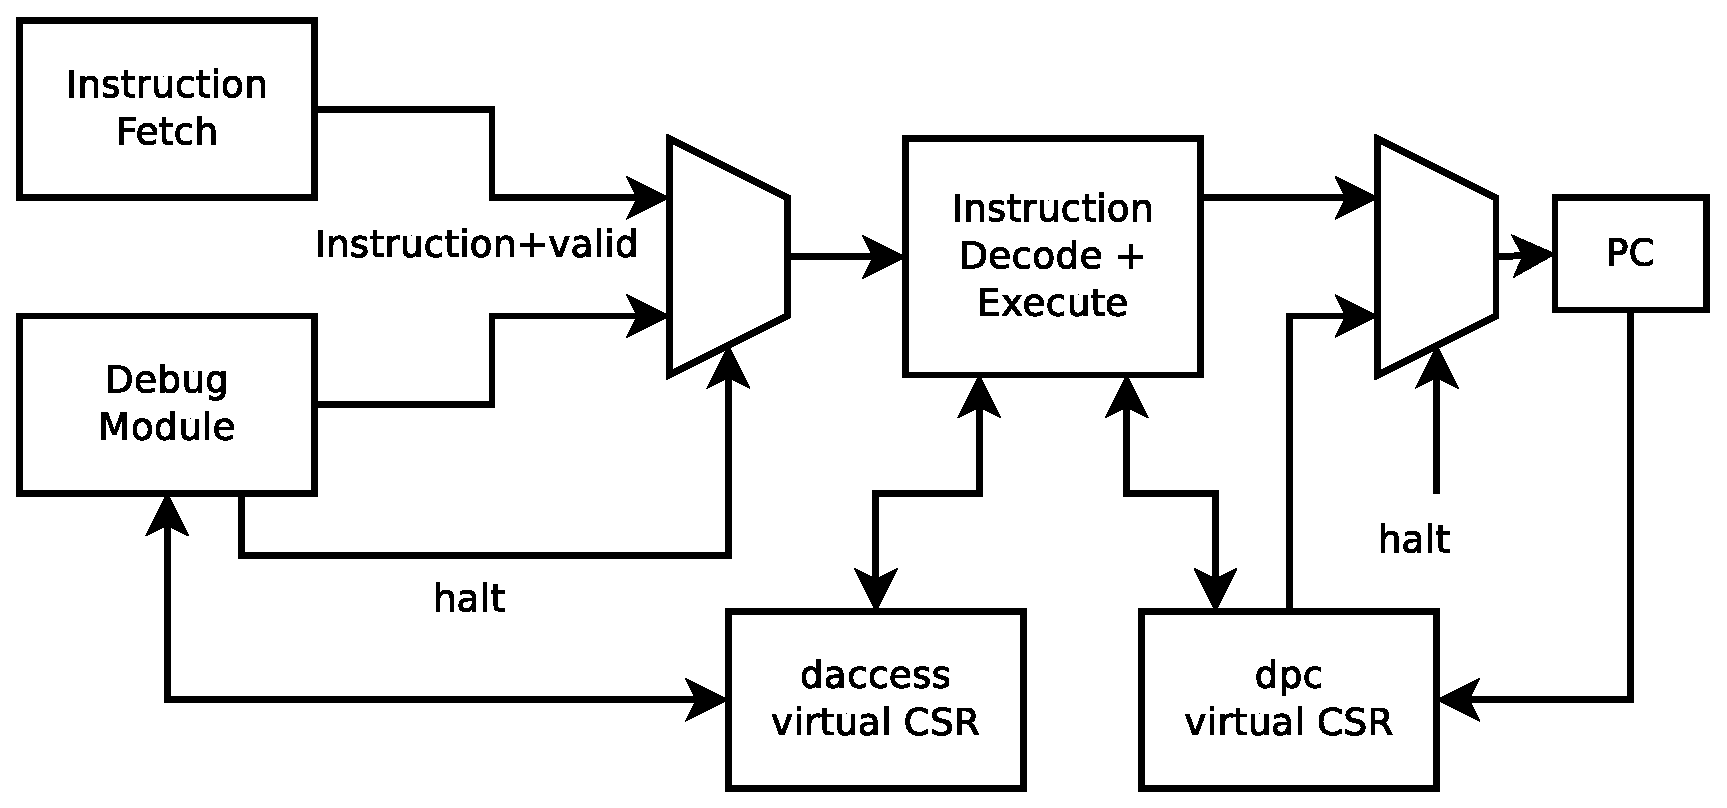
\includegraphics[width=\textwidth]{direct.eps}
   \caption{Direct Implementation}
   \label{fig:direct}
\end{figure}

Figure~\ref{fig:direct} shows an implementation that might be appropriate for
small cores.  In this implementation the DM reaches directly into the core's
pipeline to push instructions. Entering halt mode might stall the pipeline, or
send bubbles through. Data exchange happens by accessing a special CSR.
Incrementing the PC is inhibited so no separate register is needed to store the
PC. Instead accessing \Rdpc modifies the actual PC register.  When the halt is
deasserted, regular instruction execution resumes.

\subsection{Instruction Fetch}

In this implementation, just the instruction fetch unit is changed. In halt
mode the unit simply starts fetching instructions from the DM, while the PC is
unchanged. The DM could wait until the debugger gives it an instruction before
completing an access, or it could immediately return a jump-to-self instruction
if the debugger hasn't given it an instruction. Data exchange probably happens
through a special memory address. \Rdpc maps to the actual PC. When the debug
interrupt is deasserted, regular instruction execution resumes at the current
PC.

\subsection{Plain Exception}

\begin{figure}
   \centering
   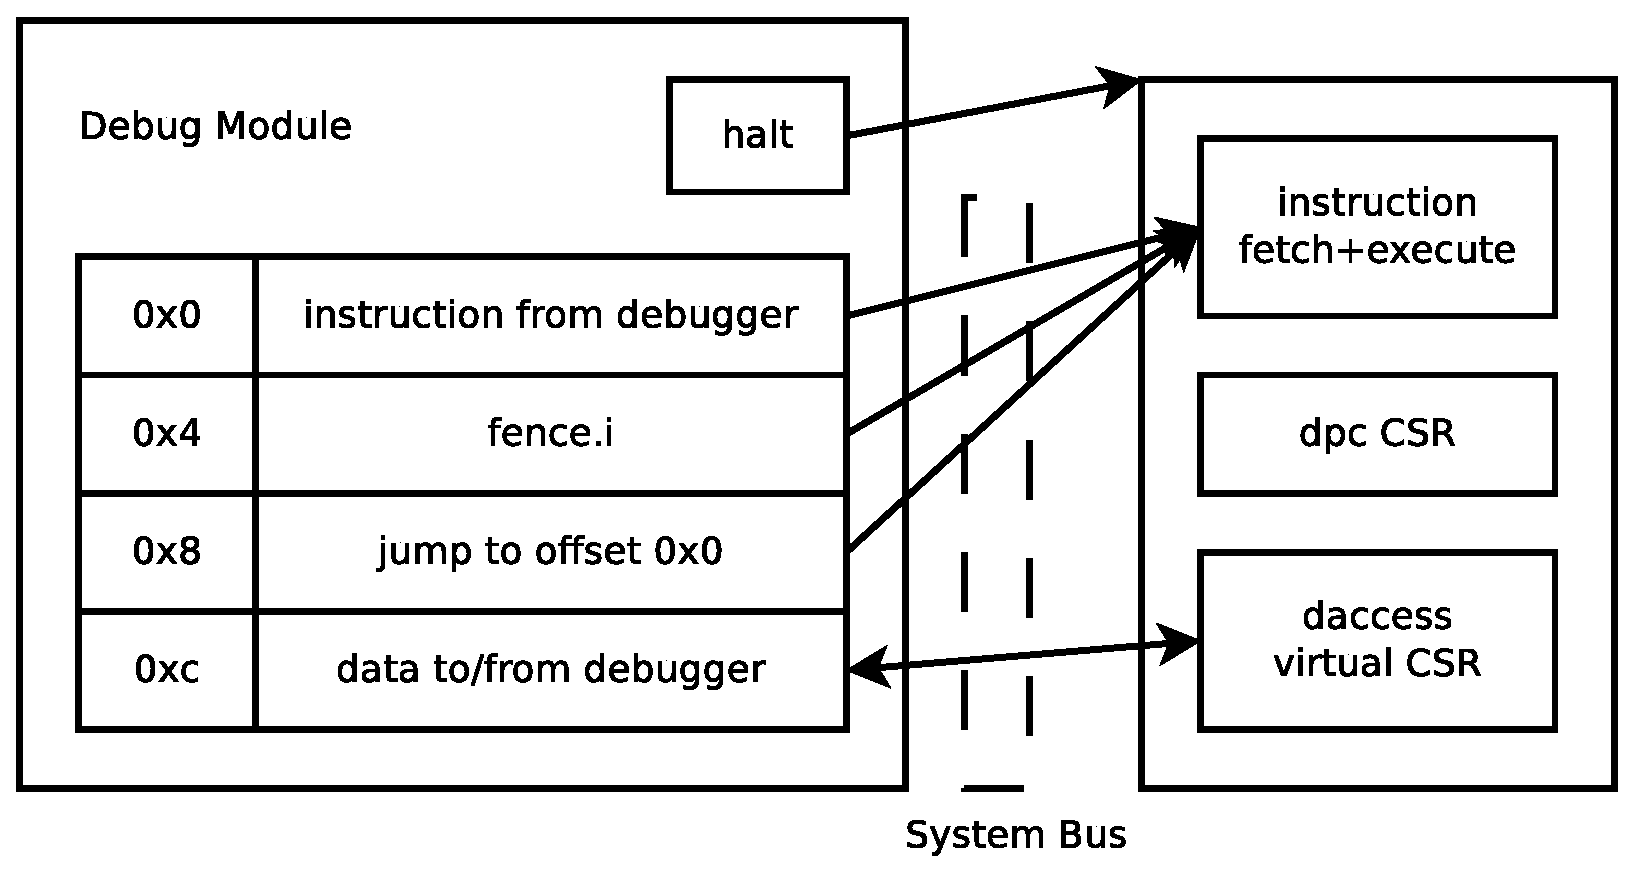
\includegraphics[width=\textwidth]{plain-exception.eps}
   \caption{Plain Exception Implementation}
   \label{fig:direct}
\end{figure}

In this implementation, being halted acts more like a real exception, jumping
to a memory region that is serviced by the DM. The PC is saved to \Rdpc. Any
details required to make the core behave correctly (eg.  executing fence.i when
a new instruction is mapped to some address) could be handled by a Debug ROM in
the DM. When the debug interrupt is deasserted, the DM feeds the hart a dret
instruction, which causes the PC to be restored and normal execution to resume.
Data is probably exchanged through a memory address.

In single-hart systems, the DM can just keep an instruction fetch access alive
until the debugger has data for it.  In multi-core systems, the DM must have
some way of allowing the debugger to choose which halted hart to send
instructions to. It could keep multiple fetches alive, or immediately return a
jump-to-self for harts that aren't the currently selected one. If it does that,
it must pretend to the debugger that there is an access pending. In the process
it assumes that a hart is going to keep fetching instructions, and won't
suddenly go to sleep or be powered down.

\section{Debugger Implementation}

This section details how an external debugger might use the described debug
interface to perform some common operations on RISC-V cores using the JTAG DTM.
All these examples assume a 32-bit core but it should be easy to adapt the
examples to 64- or 128-bit cores.

\subsection{Debug Bus Access} \label{dbusaccess}

To read an arbitrary Debug Bus register, select \Rdbus, and scan in a value
with \Fop set to 1, and \Faddress set to the desired register address. In
Update-DR the operation will start, and in Capture-DR its results will be
captured into \Fdata.  If the operation didn't complete in time, \Fop will be 3
and the value in \Fdata must be ignored. The error condition must be cleared by
writing \Fdbusreset in \Rdtmcontrol, and then the operation must be tried
again. This time the debugger should allow for more time between Capture-DR and
Update-DR.

To write an arbitrary Debug Bus register, select \Rdbus, and scan in a value
with \Fop set to 2, and \Faddress and \Fdata set to the desired register
address and data respectively. From then on everything happens exactly as with
a read, except that a write is also performed right after the read. The
operation isn't considered complete until the write has happened.

It should almost never be necessary to scan IR, avoiding a big part of the
inefficiency in typical JTAG use.

\subsection{Main Loop}

A debugger continuously monitors \Rdasum to see if any harts have spontaneously
halted.

\subsection{Data Transfer}

Depending on a core's implementation, a debugger needs to use either {\tt
csrr}/{\tt csrw} or {\tt lw}/{\tt sw} instructions to move data between GPRs
and the DM. The debugger can discover which option is required by looking at
\Rhartinfo.

This document uses the pseudo-op {\tt xmit} to indicate transfer from GPR to
the DM, and {\tt recv} to indicate transfer from DM to the GPR.

\subsection{Halting}

To halt a hart, the debugger sets \Fhartid and \Fhalt.

Once halted (as evidenced by \Faccess in \Raccess), the debugger can push
instructions to the hart by writing individual instructions to \Rifetch.

To do anything useful and non-destructive, the debugger must then save a
register (\Szero in this example), by pushing:
\begin{minted}{gas}
        xmit    s0, DM
        # Service the write data access.
\end{minted}
This causes the core to initiate a data access to the DM. The debugger sees
this happen (\Faccess in \Raccess becomes 2) and reads the register's value.
Usually the debugger will want to save an additional register (eg. \Sone).

Typically the debugger will also want to read \Rpc, by pushing:
\begin{minted}{gas}
        csrr    s0, DPC
        xmit    s0, DM
        # Service the write data access.
\end{minted}

Performing other operations all comes down to writing the appropriate
instructions, so the sections below mostly consist of short program listings.

A debugger can combine all the accesses above in a single request to the debug
adapter which the adapter executes as quickly as possible. (It's probably
limited by the TCK speed.) In that case the debugger must check \Fioverflow,
\Fdunderflow, and \Fdoverflow afterwards to confirm that all operations
completed successfully. If not then it must try the operation again, with some
delays built in.

\subsection{Reading Memory}

Push the following instructions into the hart:
\begin{minted}{gas}
        recv    s0, DM
        # Service the read data access with the address to read from.
        lw      s0, 0(s0)
        xmit    s0, DM
        # Service the write data access by reading the data that was read from
        # memory.
\end{minted}

A block of memory can be read efficiently using the Instruction Buffer. First,
load the start address of the memory block into \Sone by pushing:
\begin{minted}{gas}
        recv    s1, DM
        # Service the read data access with the address to read from.
\end{minted}

Then load the following into the Instruction Buffer:
\begin{minted}{gas}
        lw      s0, 0(s1)
        xmit    s0, DM
        addi    s1, s1, 4
\end{minted}

Enable the Instruction Buffer by asserting \Fibufenable and setting
\Fibufaction to 1. The DM will start feeding the instructions to the core. Once
it hits the {\tt xmit} pseudo-op, the core will send a word to the DM, which
the debugger sees and reads. Execution of instructions is suspended while that
access is happening.  When the debugger gets the last word that it is
interested in, it clears \Fibufenable before reading it.

Using this technique, one word can optimistically be read for every JTAG bus
access. The debugger must check \Fdunderflow afterwards to ensure it never read
too quickly. If it did, then it can retry the operation with some artificial
delays added.

Table~\ref{tab:memread} shows the scans involved in reading a single word using
this method.

\begin{table}[htp]
    \centering
    \caption{Memory Read Timeline}
    \label{tab:memread}
    \begin{tabulary}{\textwidth}{|r|l|L|}
        \hline
        & JTAG State & Activity \\
        \hline
        TODO & TODO & TODO \\
%        1 & Shift-DR & Debugger shifts in write of 0x41002403 to dram[0], and
%        gets back the result of whatever happened previously. \\
%        & Update-DR & DTM starts read from dram[0], followed by write to
%        dram[0]. \\
%        \hline
%        2 & Capture-DR & DTM captures results of read from dram[0]. \\
%        & Shift-DR & Debugger shifts in write of 0x42483 to dram[1], and gets
%        back the old contents of the first word in Debug RAM. \\
%        & Update-DR & DTM starts read from dram[1], followed by write to
%        dram[1]. \\
%        \hline
%        3 & Capture-DR & DTM captures results of read from dram[1]. \\
%        & Shift-DR & Debugger shifts in write of 0x40902823 to dram[2], and
%        gets back the old contents of the second word in Debug RAM. \\
%        & Update-DR & DTM starts read from dram[2], followed by write to
%        dram[2]. \\
%        \hline
%        4 & Capture-DR & DTM captures results of read from dram[2]. \\
%        & Shift-DR & Debugger shifts in write of 0x3f80006f to dram[3], and
%        gets back the old contents of the third word in Debug RAM. \\
%        & Update-DR & DTM starts read from dram[3], followed by write to
%        dram[3]. \\
%        \hline
%        5 & Capture-DR & DTM captures results of read from dram[3]. \\
%        & Shift-DR & Debugger shifts in write of the address the user wants to
%        read from to dram[4], using the interrupting Debug RAM register to assert
%        the Debug Interrupt. The old contents of the fourth word in Debug RAM
%        are shifted out. \\
%        & Update-DR & DTM starts read from dram[4], followed by write to
%        dram[4], and then sets the interrupt bit. The hart will respond to the
%        Debug Interrupt by executing the program in Debug RAM which in this
%        case will read the address written, and replace the entry in Debug RAM
%        with the data at that address. \\
%        \hline
%        6 & Capture-DR & DTM captures results of read from dram[4]. \\
%        & Shift-DR & Debugger shifts in read from dram[4], and gets back the
%        old contents of the fourth word in Debug RAM. (This is the value that
%        was there just before the address was written there.) \\
%        & Update-DR & DTM starts read from dram[4]. \\
%        \hline
%        7 & Capture-DR & DTM captures results of read from dram[4]. \\
%        & Shift-DR & Debugger shifts in nop, and gets back the contents of the
%        fourth word in Debug RAM. This is the value that was there during the
%        previous Update-DR, which is the result of the Debug Program execution.
%        \\
        \hline
    \end{tabulary}
\end{table}

\subsection{Writing Memory} \label{writemem}

To write a single word:
\begin{minted}{gas}
        recv    s0, DM
        # Service the data read with the address to write to.
        recv    s1, DM
        # Service the data read with the data to write.
        sw      s1, 0(s0)
\end{minted}

Similar to reading a block of memory, writing can also be done efficiently.
Load the start address of the memory block into \Sone by pushing:
\begin{minted}{gas}
        recv    s1, DM
        # Service the read data access with the address to read from.
\end{minted}

Then load the following into the Instruction Buffer:
\begin{minted}{gas}
        recv    s0, DM
        sw      s0, 0(s1)
        addi    s0, s0, 4
\end{minted}

Enable the Instruction Buffer by asserting \Fibufenable and setting
\Fibufaction to 1. The DM will start feeding the instructions to the core. Once
it hits the {\tt recv} pseudo-op, the core will wait for a word from the DM.
The debugger notices and responds.  When the debugger gets to the last word
that it is interested in, it clears \Fibufenable before completing the read
access it.

When done, the debugger must check \Fdoverflow to confirm everything went as
expected.

\begin{commentary}
    % Select-DR-Scan to Shift-DR: 2
    % Shift-DR to Exit1-DR: dbus register is abits+33 bits, so 38
    % Exit1-DR to Select-DR-Scan: 2
    % Total: 42

    TODO: maybe update

    After the instruction buffer is configured, each word can be written to the
    target in 42 TCK cycles. That's 76\% efficient, and translates to a
    download speed of 930KB/s at a 10MHz TCK.  That should be good enough that
    it's not worth making the JTAG interface more complex to improve the
    efficiency. (This assumes the Debug Bus uses 5 address bits and that the
    debugger never has to wait for the core.)
\end{commentary}

\subsection{Reading Registers}

Floating point register (\Fone):
\begin{minted}{gas}
        fmv.x.s s0, f1
        xmit    s0, DM
        # Read the actual data.
\end{minted}

CSR (\Rmepc):
\begin{minted}{gas}
        csrr    s0, MEPC
        xmit    s0, DM
        # Read the actual data.
\end{minted}

\subsection{Writing Registers} \label{writereg}

Eg. how to write \Rmepc.
\begin{minted}{gas}
        recv    s0, DM
        # Write the actual data.
        csrw    MEPC, s0
\end{minted}

\subsection{Running}

First, the debugger should restore any registers that it has clobbered.  Once
that's done, it can let the core run by clearing \Fhalt.

\subsection{Single Step}

A debugger can single step the core by setting a breakpoint on the next
instruction and letting the core run, or by asking the hardware to perform a
single step. The former requires the debugger to have much more knowledge of
the hardware than the latter, so the latter is preferred.

Using the hardware single step feature is almost the same as regular running.
The debugger just sets \Fstep in \Rdcsr before letting the core run. The core
behaves exactly as in the running case, except that interrupts are left off and
it only fetches and executes a single instruction before re-entering Debug
Mode.

\subsection{Handling Exceptions}

Generally the debugger can avoid exceptions by being careful with the programs
it writes. Sometimes they are unavoidable though, eg. if the user asks to
access memory or a CSR that is not implemented. A typical debugger will not
know enough about the platform to know what's going to happen, and must attempt
the access to determine the outcome.

When an exception occurs in Halt Mode, \Fhmexc becomes set. If the debugger did
something that might have caused an exception, it should check for that. If
there was an exception, it's left to the debugger to know what must have caused
it.

\subsection{Quick Access} \label{quickaccess}

If it's undesirable to halt a hart for more than a few milliseconds, a debugger
can perform a quick action. This requires both the Instruction Buffer and the
Scratch RAM. The Scratch RAM is accessed through the DM, either using
memory-mapped access or special CSRs.  Below we'll uses the pseudo-op {\tt
save} to indicate transfer from GPR to Scratch RAM, and {\tt restore} to
indicate transfer from Scratch RAM to the GPR.

To perform a quick memory read, the debugger first writes the following into the
Instruction Buffer:
\begin{minted}{gas}
        save    s0, SCRATCH0
        restore s0, SCRATCH1
        lw      s0, 0(s0)
        save    s0, SCRATCH1
        restore s0, SCRATCH0
\end{minted}
Then it writes the address to read from to the second word in the Scratch RAM.
Finally it asserts \Fibufenable, and sets \Fibufaction to 2. The debugger can
monitor \Fibufenable and when it's clear again, it knows the hart has executed
the instructions. At that point it can read the data value from the second word
in the Scratch RAM.

To perform a quick memory write, the debugger writes the following into the
Instruction Buffer:
\begin{minted}{gas}
        save    s0, SCRATCH0
        save    s1, SCRATCH1
        restore s0, SCRATCH2
        restore s1, SCRATCH3
        sw      s1, 0(s0)
        restore s0, SCRATCH0
        restore s1, SCRATCH1
\end{minted}
Then it writes the address to write to into the 3rd word of Scratch RAM, and
the value to write into the 4th word.  Finally it asserts \Fibufenable, and
sets \Fibufaction to 2. The debugger can monitor \Fibufenable and when it's
clear again, it knows the hart has executed the instructions.

Quick reads require a 5-instruction Instruction Buffer and a 2-word Scratch
RAM.  Quick writes require a 7-instruction Instruction Buffer and a 4-word
Scratch RAM.

\section{Trace Module}

{\bf This part of the spec needs work before it's ready to be implemented,
which is why it's in the appendix. It's left here to give a rough idea of some
of the issues to consider.}

Aside from viewing the current state of a core, knowing what happened in the
past can be incredibly helpful. Capturing an execution trace can give a user
that view.  Unfortunately processors run so fast that they generate trace data
at a very large rate. To help deal with this, the trace data format allows for
some simple compression.

The trace functionality described here aims to support 3 different use cases:
\begin{enumerate}
    \item Full reconstruction of all processor state, including register values
        etc. To achieve this goal the decoder will have to know what code is
        being executed, and know the exact behavior of every RISC-V
        instruction.
    \item Reconstruct just the instruction stream. Get enough data from the
        trace stream that it is possible to make a list of every instruction
        executed.  This is possible without knowing anything about the code or
        the core executing it.
    \item Watch memory accesses for a certain memory region.
\end{enumerate}

Trace data may be stored to a special on-core RAM, RAM on the system bus, or to
a dedicated off-chip interface. Only the system RAM destination is covered
here.

\subsection{Trace Data Format}

Trace data should be both compact and easy to generate. Ideally it's also easy
to decode, but since decoding doesn't have to happen in real time and will
usually have a powerful workstation to do the work, this is the least important
concern.

Trace data consists of a stream of 4-bit packets, which are stored in memory in
32-bit words by putting the first packet in bits 3:0 of the 32-bit word, the
second packet into bits 7:4, and so on. Trace packets and their encoding are
listed in Table~\ref{tab:tracepackets}.

\begin{table}[htp]
   \centering
   \caption{Trace Sequence Header Packets}
   \label{tab:tracepackets}
   \begin{tabulary}{\textwidth}{|l|l|L|}
      \hline
      0000 & Nop & Packet that indicates no data. The trace source must use
      these to ensure that there are 8 synchronization points in each buffer. \\
      \hline
      0001 & PC & Followed by a Value Sequence containing bits XLEN-1:1 of the
      PC if the compressed ISA is supported, or bits XLEN-1:2 of the PC if the
      compressed ISA is not supported.
      Missing bits must be filled in with the last PC value. \\
      \hline
      0010 & Branch Taken & \\
      \hline
      0011 & Branch Not Taken & \\
      \hline
      0100 & Trace Enabled & Followed by a single packet indicating the version
      of the trace data (currently 0). \\
      \hline
      0101 & Trace Disabled & Indicates that trace was purposefully disabled,
      or that some sequences were dropped because the trace buffer overflowed. \\
      \hline
      0110 & Privilege Level & Followed by a packet containing whether the
      cause of the change was an interrupt (1) or something else (0) in bit 3,
      PRV[1:0] in bits 2:1, and IE in bit 0. \\
      \hline
      0111 & Change Hart & Followed by a Value Sequence containing the hart ID
      of the hart whose trace data follows. Missing bits must be filled in with
      0. \\
      \hline
      1000 & Load Address & Followed by a Value Sequence containing the
      address.  Missing bits must be filled in with the last Load Address
      value. \\
      \hline
      1001 & Store Address & Followed by a Value Sequence containing the
      address. Missing bits must be filled in with the last Store Address
      value. \\
      \hline
      1010 & Load Data & Followed by a Value Sequence containing the data.
      Missing bits must be filled in by sign extending the value. \\
      \hline
      1011 & Store Data & Followed by a Value Sequence containing the data.
      Missing bits must be filled in by sign extending the value. \\
      \hline
      1100 & Timestamp & Followed by a Value Sequence containing the timestamp.
      Missing bits should be filled in with the last Timestamp value. \\
      \hline
      1101 & Reserved & Reserved for future standards. \\
      \hline
      1110 & Custom & Reserved for custom trace data. \\
      \hline
      1111 & Custom & Reserved for custom trace data. \\
      \hline
   \end{tabulary}
\end{table}

Several header packets are followed by a Value Sequence, which can encode
values between 4 and 64 bits. The sequence consists first of a 4-bit size
packet which contains a single number N.  It is followed by N+1 4-bit packets
which contain the value. The first packet contains bits 3:0 of the value. The
next packet contains bits 7:4, and so on.

\subsection{Trace Events}

Trace events are events that occur when a core is running that result in trace
packets being emitted. They are listed in Table~\ref{tab:traceevents}.

\begin{table}[htp]
   \centering
   \caption{Trace Data Events}
   \label{tab:traceevents}
   \begin{tabulary}{\textwidth}{|l|L|}
      \hline
      Opcode & Action \\
      \hline
      {\tt jal} & If \Femitbranch is disabled but \Femitpc is enabled, emit
      2 PC values: first the address of the instruction, then the address being
      jumped to. \\
      \hline
      {\tt jalr} & If \Femitbranch is disabled but \Femitpc is enabled, emit 2 PC
      values: first the address of the instruction, then the address being
      jumped to. Otherwise, if \Femitstoredata is enabled emit just the
      destination PC. \\
      \hline
      BRANCH & If \Femitbranch is enabled, emit either Branch Taken or Branch
      Not Taken.  Otherwise if \Femitpc is enabled and the branch is taken,
      emit 2 PC values: first the address of the branch, then the address being
      branched to. \\
      \hline
      LOAD & If \Femitloadaddr is enabled, emit the address.  If
      \Femitloaddata is enabled, emit the data that was loaded. \\
      \hline
      STORE & If \Femitstoreaddr is enabled, emit the address. If
      \Femitstoredata is enabled, emit the data that is stored. \\
      \hline
      Traps & {\tt scall}, {\tt sbreak}, {\tt ecall}, {\tt ebreak}, and {\tt
      eret} emit the same as if they were {\tt jal} instructions. In addition they
      also emit a Privilege Level sequence. \\
      \hline
      Interrupts & Emit PC (if enabled) of the last instruction executed.  Emit
      Privilege Level (if enabled).  Finally emit the new PC (if enabled). \\
      \hline
      CSR instructions & For reads emit Load Data (if enabled). For writes emit
      Store Data (if enabled). \\
      \hline
      Data Dropped & After packet sequences are dropped because data is
      generated too quickly, Trace Disabled must be emitted. It's not necessary
      to follow that up with a Trace Enabled sequence. \\
      \hline
   \end{tabulary}
\end{table}

\subsection{Synchronization}

If a trace buffer wraps, it is no longer clear what in the buffer is a header
and what isn't. To guarantee that a trace decoder can sync up easily, each
trace buffer must have 8 synchronization points, spaced evenly throughout the
buffer, with the first one at the very start of the buffer. A synchronization
point is simply an address where there is guaranteed to be a sequence header.
To make this happen, the trace source can insert a number of Nop headers into
the sequence just before writing to the synchronization point.

Aside from synchronizing a place in the data stream, it's also necessary to
send a full PC, Read Address, Write Address, and Timestamp in order for those
to be fully decoded. Ideally that happens the first time after every
synchronization point, but bandwidth might prevent that. A trace source should
attempt to send one full value for each of these (assuming they're enabled)
soon after each synchronization point.

\subsection{Trace Registers}

\input{trace_registers.tex}

\section{Future Ideas}
Some future version of this spec may implement some of the following features.

\begin{enumerate}
   \item The spec defines several additions to the Device Tree which enable a
      debugger to discover hart IDs and supported triggers for all the cores
      in the system.
   \item DTMs can function as general bus slaves, so they would look like
      regular RAM to bus masters.
   \item Harts can be divided into groups. All the harts in the same group can
      be halted/run/stepped simultaneously. When a hart hits a breakpoint, all
      the other harts in the same group also halt within a few clock cycles.
   \item DTMs are specified for protocols like USB, I2C, SPI, and SWD.
   \item Core registers can be read without halting the processor.
   \item The debugger can communicate with the power manager to power cores up
      or down, and to query their status.
   \item Serial ports can raise an interrupt when a send/receive queue becomes full/empty.
   \item The debug interrupt can be masked by running code. If the interrupt is
      asserted, then deasserted, and then asserted again the debug interrupt
      happens anyway. This mechanism can be used to eg. read/write memory with
      minimal interruption, making sure never to interrupt during a critical
      piece of code.
   \item The debugger can non-intrusively sample a recent PC value from any
      running hart.
\end{enumerate}

\section{Change Log}

\begin{versionhistory}
    \vhEntry{0.10}{Jul 11}{TN}{Version shared for 4th RISC-V Workshop}
    \vhEntry{0.11}{Jul 17}{TN}{Updated Bus Access section}
    \vhEntry{0.11}{Jul 29}{TN}{\Rmcontrol is intended to alias {\tt tdata0}.
        Remove conditional writes.}
    \vhEntry{0.11}{Aug 11}{TN}{Document {\tt wfi} behavior in Halt Mode.
        Core Debug Registers are only accessible in Halt Mode. Removed hwbpcount
        field from \Rdcsr.}
    \vhEntry{0.11}{Aug 22}{TN}{Clarify meaning of $|mode|$ in \Rtselect. All
        triggers are either locked by the debugger, or none are.}
    \vhEntry{0.11}{Aug 23}{TN}{Triggers are locked on an individual basis
        again. See \Fdmode in {\tt tdata0}. The definitions of \Fchain in
        \Rmcontrol has been changed to be easier to explain. Changed
        recommendations on when store hardware breakpoints fire.}
    \vhEntry{0.11}{Aug 25}{TN}{Add \Ftiming to \Rmcontrol. Changed
        encoding of \Faction.}
    \vhEntry{0.11}{Aug 26}{TN}{Document {\tt lr}/{\tt sc} behavior.
        Rename {\tt tdata0}--{\tt tdata2} to {\tt tdata1}--{\tt tdata3}.}
    \vhEntry{0.11}{Sep 6}{TN}{Change Debug Bus to only support simple
        read and write operations.}
    \vhEntry{0.11}{Sep 7}{TN}{Clarify \Fop in \Rdbus.}
    \vhEntry{0.11}{Sep 13}{TN}{Add rough idea of instruction count
        triggers that could be used for single step.}
    \vhEntry{0.11}{Sep 27}{TN}{M-mode writes to triggers with dmode=1 are
        ignored instead of raising an exception.}
    \vhEntry{0.11}{Oct 24}{TN}{Change serial full bit to full/overflow.}
    \vhEntry{0.11}{Nov 2}{TN}{There actually can be side effects to reading
        Debug Bus registers (specifically reading serial data).}
    \vhEntry{0.12}{Nov 10}{TN}{Reduce Debug Bus width to 32 bits. This
        caused a lot of changes in Section~\ref{dm}, and some in
        Section~\ref{dbus}. Read Section~\ref{dbusaccess} to get an idea of how
        that affects the debugger.}
\end{versionhistory}

\end{document}
